\section{Casos de Estudo}
\label{sec:chap03_marketstudy}
A investigação neste campo de estudo tem vindo a desenvolver-se desde o século XX~\parencite{survey_nlidb}. Assim sendo, é importante apresentar e examinar os casos mais pertinentes para o protótipo em desenvolvimento neste trabalho, na perspetiva de perceber quais as inovações que cada um deles trouxe para a área das \glspl{ilnbd} e em que medida se enquadram com o problema em resolução.

\subsection{LUNAR}
O LUNAR é um sistema que dá resposta ao domínio de amostras de rochas trazidas da lua e foi o primeiro sistema \gls{ilnbd}~\parencite{nlidb_brief_review, survey_nlidb}. O desenvolvimento deste sistema surgiu da necessidade de possibilitar aos cientistas envolvidos no estudo das rochas lunares poderem obter informação para formular e testar as suas hipóteses, de uma forma simples e intuitiva. O LUNAR permitia ao cientista executar diversas ações como fazer questões, computar médias e taxas, criar listas baseadas em critérios de seleção ou comparar medidas de diferentes investigadores, usando informação de duas bases de dados, uma contendo dados de análises químicas e a outra com dados de referências bibliográficas. Apesar de ter sido desenvolvido como protótipo, este sistema apresentou um desempenho satisfatório, sendo que cerca de 78\% dos pedidos foram respondidos com sucesso~\parencite{lunar_sciences_nlis}.

\subsection{LADDER}
O LADDER é um sistema desenhado para consultar informação sobre navios da Marinha Americana, por forma a auxiliar os gestores da Marinha no processo de tomada de decisão~\parencite{nlidb_brief_review, developing_nli_complex_data}. O sistema, que usa gramática semântica para tratar \textit{queries} a uma base de dados distribuída, apresenta uma arquitetura de três camadas, cada uma correspondente a um componente do sistema: o INLAND -- \textit{Infomal Natural Language Access to Navy Data} --, é responsável por aceitar a \textit{query} de linguagem natural, produzir a respetiva \textit{query} de base de dados a partir da decomposição da mesma em fragmentos, sendo posteriormente combinados para unidades sintáticas a alto nível, para que sejam reconhecidas, dando origem a um comando enviado para o próximo componente; o IDA -- \textit{Intelligent Data Access} --, compõe uma resposta com base no comando recebido e organiza a sequência correta de \textit{queries} a realizar; o FAM -- \textit{File Access Manager} --, o último componente, tem a responsabilidade de gerir o acesso à base de dados distribuída~\parencite{developing_nli_complex_data}.

\subsection{CHAT-80}
Segundo \textcite{nlidb_brief_review}, o CHAT-80 é um dos sistemas \gls{pln} mais referenciados nos anos 80. O CHAT-80 foi desenvolvido pensando na adaptabilidade a diversos domínios, de forma fácil e eficiente. Foi implementado em \textit{Prolog} e incluía uma base de conhecimento com factos geográficos de mais de 150 países (domínio de geografia mundial) e vocabulário inglês suficiente para interação com uma base de dados, que neste caso específico seria implementada totalmente em \textit{Prolog}. Os autores concordaram que a aplicação devia lidar com um conjunto restrito de linguagem natural relevante para o domínio, uma vez que dessa forma se torna uma linguagem de \textit{query} formal mas acessível para o utilizador~\parencite{efficient_easily_adaptable_system_interpreting_nlq}.

\subsection{JANUS}
O JANUS é uma aplicação \gls{pln} com a capacidade de \inquotes{comunicar} com múltiplos sistemas, tais como bases de dados, sistemas periciais, dispositivos gráficos, sendo capaz de avaliar a \textit{query} de linguagem natural e inferir acerca de quais os recursos a utilizar, sem que o utilizador se apercebesse da complexidade do sistema~\parencite{nlidb_brief_review, access_multiple_underlying_system_janus}. O fluxo do JANUS consistia em extrair as expressões da \textit{query} de linguagem natural, usando uma linguagem desenvolvida para o efeito, denominada \textit{World Model Language}; traduzir essas expressões para uma representação simplificada e normalizada; aplicar o algoritmo desenvolvido para encontrar a combinação adequada de serviços a disponibilizar, de modo a satisfazer o pedido do utilizador; por fim, a criação e execução de um plano para extração da informação~\parencite{access_multiple_underlying_system_janus}.

\subsection{PRECISE}
O PRECISE é um sistema desenvolvido na Universidade de Washington, cuja base de dados alvo é relacional, usando \gls{sql}, e que introduz o conceito de frases semanticamente tratáveis, ou seja, \textit{queries} que podem ser traduzidas para uma representação semântica única~\parencite{overview_nlidb_approaches_implementation_airline, nlidb_brief_review}.

\subsection{NALIX}
O NALIX -- \textit{Natural Language Interface for an XML Database} -- é uma \gls{ilnbd} desenvolvida na Universidade de Michigan, com o intuito de obter informação genérica a partir de uma base de dados em \gls{xml}~\parencite{nalix_interactive_nli_querying_xml}. De acordo com~\textcite{nalix_interactive_nli_querying_xml}, o desafio consiste em traduzir uma \textit{query} de linguagem natural para uma \textit{query} corretamente estruturada para uso numa base de dados, permitindo assim ao utilizador usar operações complexas (\exempligratia{agregação, combinação, junção, entre outras}). 

Relativamente à arquitetura do NALIX (Figura~\ref{fig:nalix_architecture}), o sistema consiste em duas partes: a primeira é responsável pela tradução da \textit{query} de linguagem natural para XQuery\footnote{Disponível em \url{https://www.w3schools.com/xml/xquery_intro.asp}.}, envolvendo os componentes \textit{Parse Tree Classifier}, \textit{Parse Tree Validator} e \textit{Parse Tree Translator}; a segunda suporta a formulação da \textit{query} de base de dados correspondente, usando os componentes \textit{Query Repository} e \textit{Message Generator}~\parencite{nalix_interactive_nli_querying_xml}.

\begin{figure}[!ht]
    \centering
    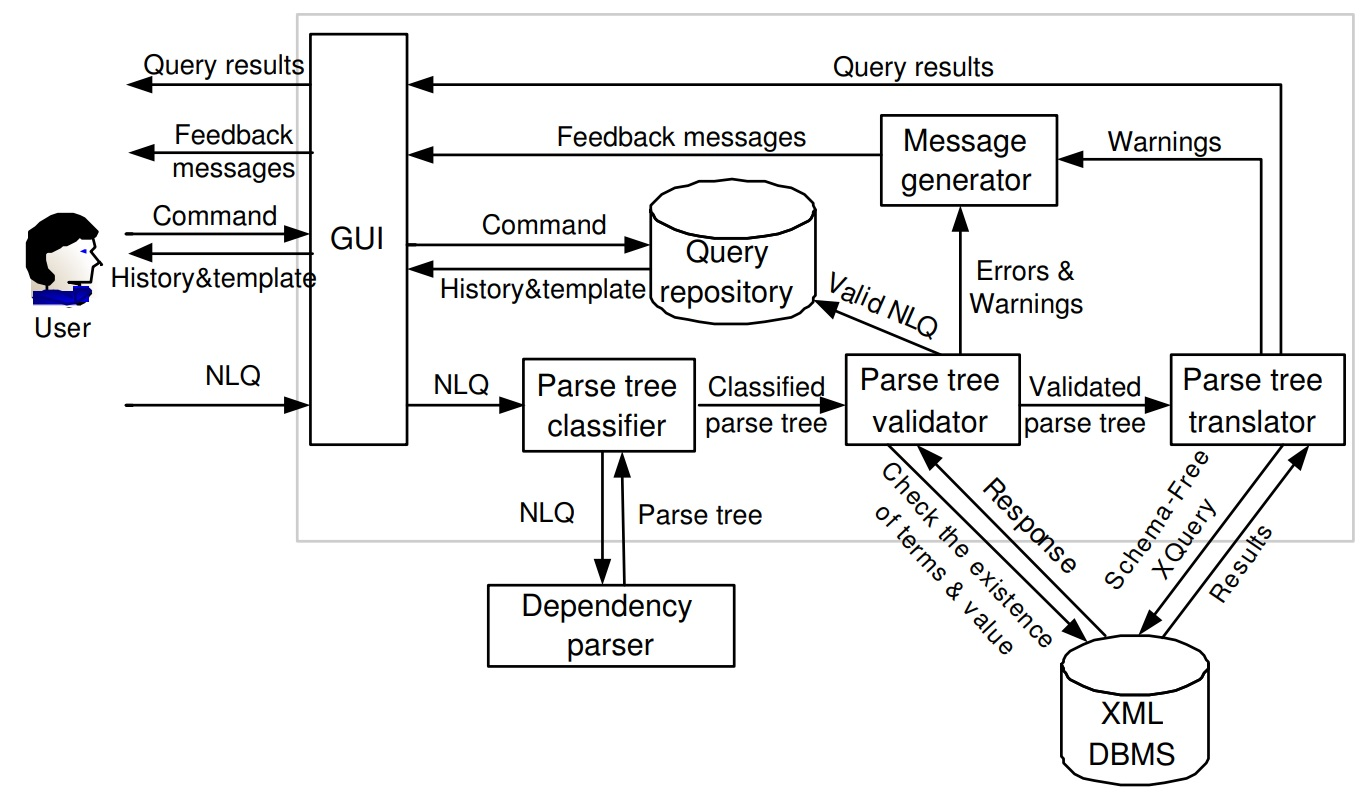
\includegraphics[width=.9\textwidth]{ch03/assets/nalix_architecture.jpg}
    \caption{Arquitetura do sistema NALIX, extraído de~\textcite{nalix_interactive_nli_querying_xml}}
    \label{fig:nalix_architecture}
\end{figure}

De salientar é que a linguagem de \textit{query} usada pelo NALIX (\textit{Schema Free XQuery}) não necessita que seja explicitado qual o \textit{schema} a ser usado, sendo que é capaz de encontrar automaticamente, para uma dada coleção de expressões/palavras-chave, todas as relações existentes entre estes elementos. Assim, é possível abstrair o sistema do domínio existente~\parencite{nalix_interactive_nli_querying_xml, survey_nlidb}.

\subsection{GINLIDB}
\tbd

\subsection{Sumário do Casos de Estudo}
\tbd